\label {sec:fs-optimization-experiments}
In this section, we describe the preliminary experiments that we conducted in order to show how the choice of a query plan affects the performance. First, we present the experiment setup and the configuration used; then, we demonstrate our results.

\subsection{Setup}

For our experiments, we used the same query that was described in Section \ref{sec:fs-optimization-problem-statement} and the Apache Beam implementation of the NEXMark benchmark model. In this implementation, each entity (\texttt{Person}, \texttt{Auction}, or \texttt{Bid}) is represented via a subclass of the \texttt{Event} class. Each event is generated by an unbounded source in accordance to the provided configuration, which includes parameters such as the arrival rate for each event, the $|Person|:|Auction|:|Bid|$ ratio, the time-based window size, etc. 

First, we execute this query using the plan in which \texttt{Auction} and \texttt{Person} are joined first, and the result is joined with \texttt{Bid}; then, we use the plan in which \texttt{Person} and \texttt{Bid} are joined first (see Section  \ref{sec:fs-optimization-problem-statement}). For each run, we use a different $|Person|:|Auction|:|Bid|$ ratio.

To evaluate performance, we measure the the latency and the throughput for each window. For a join result, we consider the \textit{latency} to be the difference between the maximum arrival time of each of the rows making up the join result and the output time of the resulting row; then, we select the maximum out of the latency values of all the rows in each window. We calculate \textit{throughput} as the ratio of execution time to the number of the elements. Additionally, we measure the correspondence between window size and latency.

\subsection{Running configuration}
We have conducted our experiments on a local machine equipped with a 1.4 GHz Intel Core i5-8257U CPU (4 cores) and 8 GB of memory using the Apache Flink runner. We plan to repeat the same experiments on a distributed system.

\subsection{Results}

In the subsequent text the plan which joins \texttt{Auction} and \texttt{Person} first is referred to as \textit{Plan 1}; the plan which joins \texttt{Person} and \texttt{Bid} first is \textit{Plan 2}.
\subsubsection{Latency}

We generated 1000000 events with the arrival rate of 10000 events per second and time-based windows of varying sizes.

As Figure \ref{fig:latency_against_window_size} demonstrates, the latency does not grow linearly as the window size increases. This is due to the fact that the join operator processes the records as they arrive instead of starting to process them only after the last record in the window has arrived, and thus the results are ready to emerge shortly thereafter the arrival of the last record in the window.

Figure \ref{fig:latency_diff_against_window_size} demonstrates how the difference in latency for the two execution plans changes with the window size. Since the difference grows as the window size increases, statistics-based optimization should provide an even bigger performance gain for larger windows.

% TODO rewrite this. first reread this then rewrite this.
Figure \ref{fig:latency_ratio} demonstrates how query execution time changes depending on data characteristics. The $|Person|:|Auction|:|Bid|$ ratio impacts arrival rate for each kind of entities, thereby influencing join execution time. As expected, the plan in which \texttt{Person} and \texttt{Auction} are joined first delivers better results when the arrival rate of \texttt{Bid} records significantly overwhelms the rates of \texttt{Person} and \texttt{Auction} (the 5:5:90 ratio is an example of such a case), while the plan in which \texttt{Person} and \texttt{Bid} are joined first works best for cases where the rate of \texttt{Auction} records far exceeds those of \texttt{Person} and \texttt{Bid}. 


\subsubsection{Throughput}

The parameters for throughput estimation were the same as for the latency estimation. As Figure \ref{fig:throughput_against_window_size} shows, 


\begin{figure}
\centering
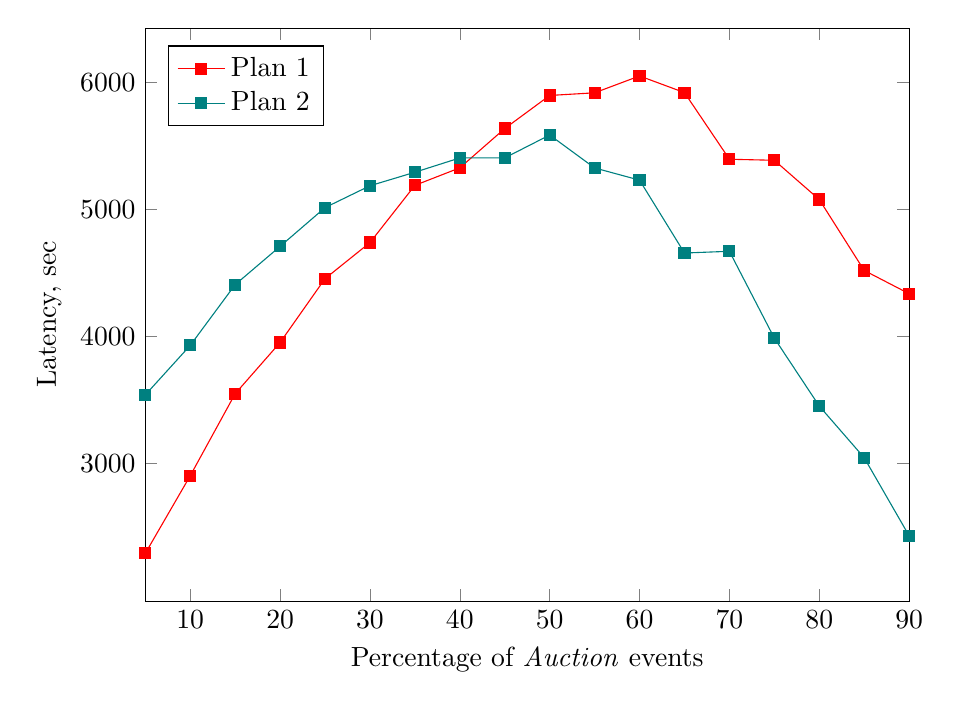
\begin{tikzpicture}
\begin{axis}[
    scale only axis=true,
    width=0.8\textwidth,
    height=0.6\textwidth,
    ytick={3000, 4000, 5000, 6000},
    yticklabels={3000, 4000, 5000, 6000},
    xmin=5, xmax=90,
    legend cell align=left,
    legend pos=north west,
    xlabel={Percentage of \textit{Auction} events},
    ylabel={Latency, sec},
    % x label style={at={(axis description cs:0.5,0.05)},anchor=north},
    % y label style={at={(axis description cs:0.125,0.5)},anchor=center},
]
\addplot[red,mark=square*,mark options={scale=1,solid}] coordinates {
    (5, 2294.73)
    (10, 2905.51)
    (15, 3550.93)
    (20, 3953.99)
    (25, 4456.47)
    (30, 4740.31)
    (35, 5190.68)
    (40, 5328.49)
    (45, 5637.89)
    (50, 5898.18)
    (55, 5918.89)
    (60, 6051.56)
    (65, 5920.56)
    (70, 5396.14)
    (75, 5387.98)
    (80, 5079.04)
    (85, 4520.84)
    (90, 4338.02)
};
\addplot[teal,mark=square*,mark options={scale=1,solid}] coordinates {
    (5, 3541.78)
    (10, 3931.32)
    (15, 4409.38)
    (20, 4710.69)
    (25, 5015.49)
    (30, 5187.45)
    (35, 5293.89)
    (40, 5406.6)
    (45, 5406.6)
    (50, 5586.84)
    (55, 5327.64)
    (60, 5231.65)
    (65, 4658.23)
    (70, 4671.75)
    (75, 3988.29)
    (80, 3453.75)
    (85, 3047.15)
    (90, 2432.85)
};
\legend{
    Plan 1\\
    Plan 2\\
}
\end{axis}
\end{tikzpicture}
\caption{Latency plotted against different $|Person|:|Auction|:|Bid|$ ratios, with $|Person|$ fixed at 5, values of $|Auction|$ on the $x$ axis, $|Bid| = 95 - |Auction|$.} 
\label{fig:latency_ratio}
\end{figure}


\begin{figure}
\centering
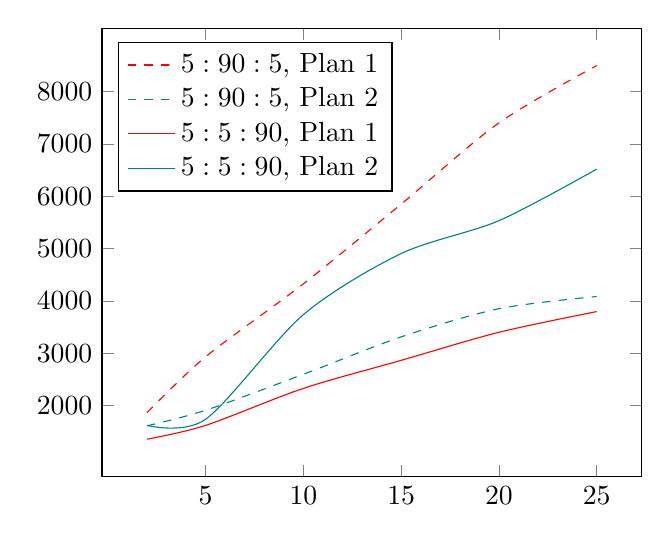
\begin{tikzpicture}
\begin{axis}[
    ytick={2000, 3000, 4000, 5000, 6000, 7000, 8000},
    yticklabels={$2000$, $3000$, $4000$, $5000$, $6000$, $7000$, $8000$},
    xtick={5, 10, 15, 20, 25},
    xticklabels={$5$, $10$, $15$, $20$, $25$},
    legend cell align=left,
    legend pos=north west
]
\addplot[smooth, red, dashed] coordinates {
(2,1864.23)
(5,2933.28)
(10,4327.74)
(15,5850.70)
(20,7403.71)
(25,8498.8)
};
\addplot[smooth, teal, dashed] coordinates {
(2,1612.74)
(5,1911.15)
(10,2598.16)
(15,3312.47)
(20,3851.92)
(25,4083.96)
};
\addplot[smooth, red] coordinates {
(2,1357.67)
(5,1621.52)
(10,2328.99)
(15,2864.79)
(20,3400.97)
(25,3796.8)
};
\addplot[smooth, teal] coordinates {
(2,1621.52)
(5,1739.10)
(10,3738.63)
(15,4905.88)
(20,5534.47)
(25,6519.64)
};
\legend{
    $5:90:5$, Plan 1\\
    $5:90:5$, Plan 2\\
    $5:5:90$, Plan 1\\
    $5:5:90$, Plan 2\\
}
\end{axis}
\end{tikzpicture}
\caption{Latency plotted against window size for different $|Person|:|Auction|:|Bid|$ ratios and execution plans.}
\label{fig:latency_against_window_size}
\end{figure}


\begin{figure}
\centering
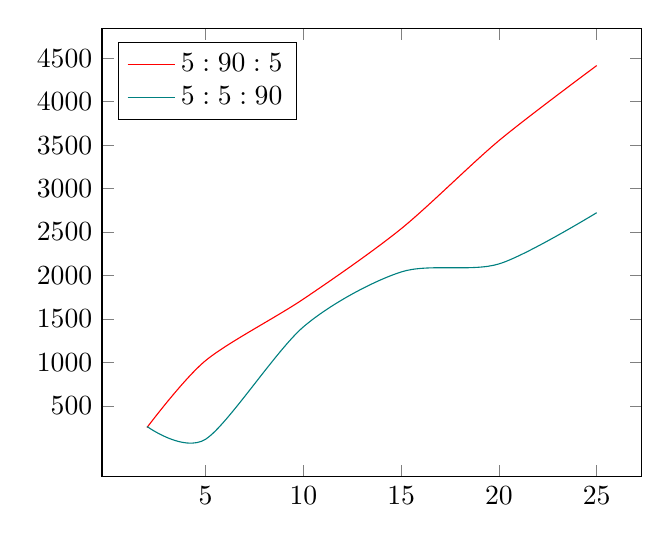
\begin{tikzpicture}
\begin{axis}[
    ytick={500, 1000, 1500, 2000, 2500, 3000, 3500, 4000, 4500},
    yticklabels={$500$, $1000$, $1500$, $2000$, $2500$, $3000$, $3500$, $4000$, $4500$},
    xtick={5, 10, 15, 20, 25},
    xticklabels={$5$, $10$, $15$, $20$, $25$},
    legend cell align=left,
    legend pos=north west
]
\addplot[smooth, red] coordinates {
(2,251.49)
(5,1022.13)
(10,1729.58)
(15,2538.23)
(20,3551.79)
(25,4414.84)
};
\addplot[smooth, teal] coordinates {
(2,263.85)
(5,117.58)
(10,1409.64)
(15,2041.09)
(20,2133.5)
(25,2722.84)
};
\legend{
    $5:90:5$\\
    $5:5:90$\\
}
\end{axis}
\end{tikzpicture}
\caption{The difference in latency for the two execution plans plotted against window size.}

\label{fig:latency_diff_against_window_size}
\end{figure}

\begin{figure}
\centering
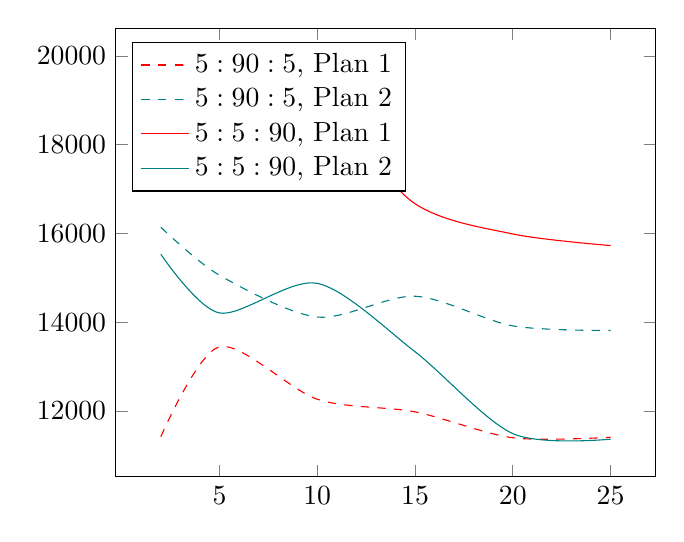
\begin{tikzpicture}
\begin{axis}[
    ytick={12000, 14000, 16000, 18000, 20000},
    yticklabels={$12000$, $14000$, $16000$, $18000$, $20000$},
    xtick={5, 10, 15, 20, 25},
    xticklabels={$5$, $10$, $15$, $20$, $25$},
    legend cell align=left,
    legend pos=north west,
    scaled ticks=false
]
\addplot[smooth, red, dashed] coordinates {
(2,11421.0)
(5,13448.3)
(10,12266.0)
(15,11981.5)
(20,11397.3)
(25,11408.4)
};
\addplot[smooth, teal, dashed] coordinates {
(2,16142.1)
(5,15059.3)
(10,14117.7)
(15,14586.4)
(20,13918.5)
(25,13813.9)
};
\addplot[smooth, red] coordinates {
(2,19782.8)
(5,19500.8)
(10,18924.7)
(15,16671.4)
(20,15989.5)
(25,15727.7)
};
\addplot[smooth, teal] coordinates {
(2,15532.8)
(5,14209.6)
(10,14876.5)
(15,13336.4)
(20,11491.7)
(25,11365.6)
};
\legend{
    $5:90:5$, Plan 1\\
    $5:90:5$, Plan 2\\
    $5:5:90$, Plan 1\\
    $5:5:90$, Plan 2\\
}
\end{axis}
\end{tikzpicture}
\caption{Throughput plotted against window size for different $|Person|:|Auction|:|Bid|$ ratios and execution plans.}
\label{fig:throughput_against_window_size}
\end{figure}


\subsection{Discussion}

The results of our experiments demonstrate that streaming query execution performance depends on the plan used for the execution, and the optimality of the plan depends on the data characteristics, which proves the necessity of adaptive optimization of streaming queries. Particularly, the first steps towards adaptive optimization should be predicting statistics for each window and performing runtime graph migration, since the results of the experiments show that even the current planners, such as the Volcano query planner \cite{graefe1993volcano} used in Apache Calcite, which are unaware of whether the data comes from a stream or a table, could use those statistics to produce a better execution plan. These two challenges will be the focus of our future work. After that, the planner can be enhanced by introducing distributed streaming systems-specific operators and their costs.



% запрос выполняется многократно на каждом окне заново и поэтому легче собирать статистику и по ней учиться